\begin{frame}
\frametitle{Introducci\'on}
Se tiene un sistema clasificador con distintos modelos en paralelo. Cada uno de esos modelos mira features de los datos y devuelve una clase. Luego se fusionan sus resultados mediante alg\'un m\'etodo, resultando en que el sistema determina la clase del dato de forma un\'ivoca. \\
\vspace{3mm}
Particularmente, el sistema resuelve problemas de clasificaci\'on binaria.
\end{frame}



\begin{frame}
\frametitle{Introducci\'on}
\begin{center}
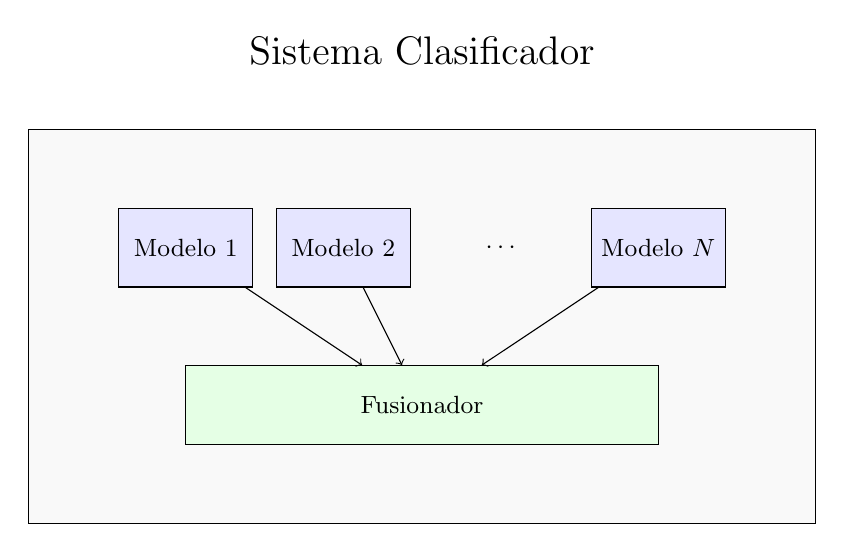
\begin{tikzpicture}[
    every node/.style={font=\small},
    modelo/.style={draw, fill=blue!10, minimum width=1.7cm, minimum height=1cm},
    fusionador/.style={draw, fill=green!10, minimum width=6cm, minimum height=1cm},
    sistema/.style={draw, fill=gray!5}
]
% Sistema
\node[sistema, minimum width=10cm, minimum height=5cm] (sistema) at (0,0) {};
\node[font=\Large] (titulo) at (0,3.5) {Sistema Clasificador};
% Modelos
\node[modelo] (modelo1) at (-3,1) {Modelo 1};
\node[modelo] (modelo2) at (-1,1) {Modelo 2};
\node at (1,1) {$\cdots$};
\node[modelo] (modeloN) at (3,1) {Modelo $N$};
% Fusionador
\node[fusionador] (fusionador) at (0,-1) {Fusionador};
% Aristas
\draw[->] (modelo1) to (fusionador);
\draw[->] (modelo2) to (fusionador);
\draw[->] (modeloN) to (fusionador);
\end{tikzpicture}
\end{center}
\end{frame}



\begin{frame}
\frametitle{Sistema ejemplo}
\begin{center}
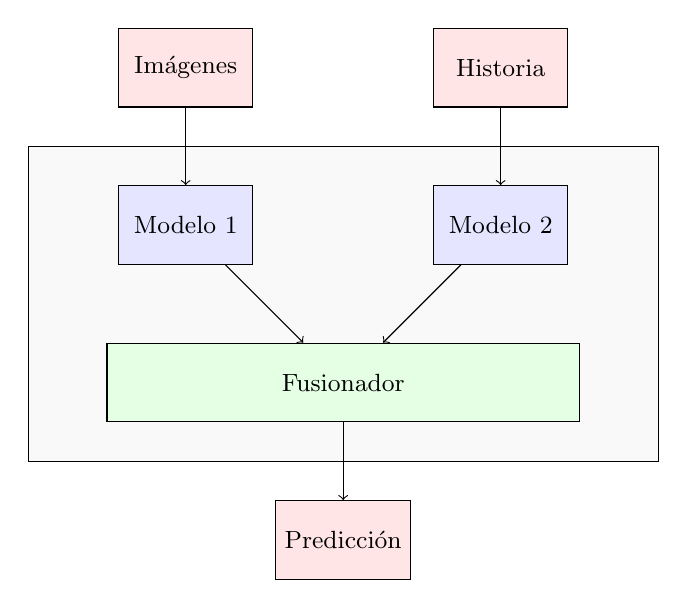
\begin{tikzpicture}[
every node/.style={font=\small},
datos/.style={draw, fill=red!10, minimum width=1.7cm, minimum height=1cm},
modelo/.style={draw, fill=blue!10, minimum width=1.7cm, minimum height=1cm},
fusionador/.style={draw, fill=green!10, minimum width=6cm, minimum height=1cm},
sistema/.style={draw, fill=gray!5}
]
% Datos
\node[datos] (datos1) at (-2,3) {Im\'agenes};
\node[datos] (datos2) at (2,3) {Historia};
% Sistema
\node[sistema, minimum width=8cm, minimum height=4cm] (sistema) at (0,0) {};
% Modelos
\node[modelo] (modelo1) at (-2,1) {Modelo 1};
\node[modelo] (modelo2) at (2,1) {Modelo 2};
% Fusionador
\node[fusionador] (fusionador) at (0,-1) {Fusionador};
% Salida
\node[datos] (resultado) at (0,-3) {Predicci\'on};
% Aristas
\draw[->] (datos1) to (modelo1);
\draw[->] (datos2) to (modelo2);
\draw[->] (modelo1) to (fusionador);
\draw[->] (modelo2) to (fusionador);
\draw[->] (fusionador) to (resultado);
\end{tikzpicture}
\end{center}
\end{frame}



\begin{frame}
\frametitle{Objetivo}
\begin{itemize}
\item Evaluar un modelo de forma independiente al sistema
\item Obtener una estimaci\'on \'util del comportamiento que tendr\'a el sistema con ese modelo
\end{itemize}
\end{frame}



\begin{frame}
\frametitle{Objetivo}
\begin{center}
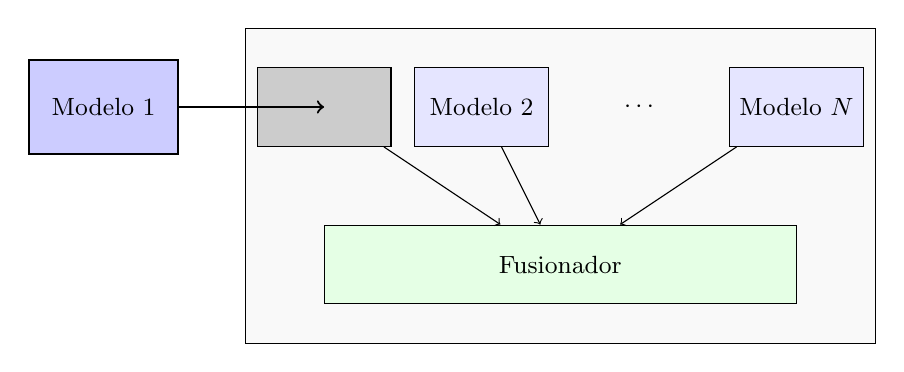
\begin{tikzpicture}[
    every node/.style={font=\small},
    modelo/.style={draw, fill=blue!10, minimum width=1.7cm, minimum height=1cm},
    fusionador/.style={draw, fill=green!10, minimum width=6cm, minimum height=1cm},
    sistema/.style={draw, fill=gray!5}
]
% Modelo externo
\node[modelo, fill=blue!20, thick, minimum width=1.9cm, minimum height=1.2cm] (modeloEvaluar) at (-5.8,1) {Modelo 1};
% Sistema
\node[sistema, minimum width=8cm, minimum height=4cm] (sistema) at (0,0) {};
% Modelos
\node[modelo, fill=gray!40] (modelo1) at (-3,1) {};
\node[modelo] (modelo2) at (-1,1) {Modelo 2};
\node at (1,1) {$\cdots$};
\node[modelo] (modeloN) at (3,1) {Modelo $N$};
% Fusionador
\node[fusionador] (fusionador) at (0,-1) {Fusionador};
% Aristas
\draw[->] (modelo1) to (fusionador);
\draw[->] (modelo2) to (fusionador);
\draw[->] (modeloN) to (fusionador);
\draw[->, thick]  (modeloEvaluar) to (-3,1);
\end{tikzpicture}
\end{center}
\end{frame}



\begin{frame}
\frametitle{Informaci\'on disponible}
Datos de los que se dispone para el problema:\\
\vspace{3mm}
\begin{itemize}
\item El sistema incompleto, faltando un modelo
\item Una funci\'on de costo para el sistema
\item Datos para la evaluaci\'on del sistema
\item El modelo a evaluar
\item Datos para la evaluaci\'on del modelo
\end{itemize}
\end{frame}



\begin{frame}
\frametitle{Informaci\'on disponible}
\begin{itemize}
\item Ambos conjuntos de datos pueden o no ser el mismo.
\item La funci\'on de costo del modelo es la que se busca proponer, y es dependiente de la funci\'on de costo del sistema y de la influencia del modelo en el sistema.
\end{itemize}
\end{frame}



\begin{frame}
\frametitle{Motivaci\'on}
Una posible utilidad de una funci\'on de costo para el modelo que sea independiente del sistema puede ser realizar b\'usqueda de hiperpar\'ametros. \\
\vspace{3mm}
Se puede querer reemplazar o añadir un modelo al sistema. Al momento de realizar la b\'usqueda de hiperpar\'ametros en el modelo, con un costo para el modelo independiente al sistema se puede comparar entre modelos de forma mucho mas r\'apida y asi elegir a los m\'as adecuados.
\end{frame}



% \begin{frame}
% \frametitle{Redes Bayesianas}
% La forma que se va a utilizar para modelar el problema es mediante una red bayesiana causal. Una red bayesiana causal es un DAG que se usa para representar distribuci\'ones probabilisticas sobre variables no independientes. Se tienen nodos para representar entidades, y aristas que representan causalidad entre esas entidades. Los nodos con doble c\'irculo son determin\'isticos dados los padres.
% \end{frame}



% \begin{frame}
% \frametitle{Redes Bayesianas}
% \centering
% \begin{tikzpicture}[scale=0.7, every node/.style={font=\tiny}]
% % Nodos
% \node[draw, fill=blue!30, minimum width=4.2cm, minimum height=3.3cm] at (0,5) (Sistema) {}; 
% \node[latent, font=\tiny, fill=green!10] at (0,10) (Persona) {$Persona$};
% \node[latent, double, font=\tiny, fill=green!40] at (3.5,8.5) (Clase) {$Clase$};
% \node[latent, font=\tiny, fill=green!10] at (-1,8) (Imagen) {$Imagen$};
% \node[latent, font=\tiny, fill=green!10] at (1,8) (Historia) {$Historia$};
% \node[latent, font=\tiny, fill=blue!20] at (-1,6) (Pred M1) {$Pred^{M1}$};
% \node[latent, font=\tiny, fill=blue!20] at (1,6) (Pred M2) {$Pred^{M2}$};
% \node[latent, double, font=\tiny, fill=blue!10] at (-2,4) (Conf M1) {$Conf^{M1}$};
% \node[latent, double, font=\tiny, fill=blue!10] at (2,4) (Conf M2) {$Conf^{M2}$};
% \node[latent, font=\tiny, fill=red!20] at (0,2) (Pred S) {$Pred^S$};
% \node[latent, double, font=\tiny, fill=red!10] at (0,0) (Conf S) {$Conf^S$};
% \node at (0,3.5) (Fusionador) {\textbf{fusionador}};
% \node[font=\large] at (-5.5,5) (Descripcion Sistema) {\color{blue} \underline{Sistema}};
% % Aristas
% \draw[->] (Persona) to (Clase);
% \draw[->] (Persona) to (Imagen);
% \draw[->] (Persona) to (Historia);
% \draw[->] (Imagen) to node[left] {\textbf{modelo 1}} (Pred M1);
% \draw[->] (Historia) to node[right] {\textbf{modelo 2}} (Pred M2);
% \draw[->] (Pred M1) to (Conf M1);
% \draw[->] (Pred M2) to (Conf M2);
% \draw[->] (Pred M1) to (Pred S);
% \draw[->] (Pred M2) to (Pred S);
% \draw[->] (Pred S) to (Conf S);
% \draw[->] (Clase) to[bend left] (Conf M1.east);
% \draw[->] (Clase.280) to[bend left] (Conf M2.north east);
% \draw[->] (Clase.south east) to[bend left] (Conf S.east);
% \draw[->, very thick, fill=blue, draw=blue] (Descripcion Sistema.east) to (Sistema.west);
% \end{tikzpicture}
% \end{frame}



\begin{frame}
\frametitle{Intervenci\'on}
Se va a utilizar una operaci\'on sobre el sistema llamada intervenci\'on, basada en la intervenci\'on de las redes bayesianas. \\
\vspace{3mm}
Al sistema sin el modelo se le inserta en ese lugar un modelo simple que hace siempre lo mismo a pesar del dato de entrada para poder analizar su comportamiento. \\
\end{frame}



\begin{frame}
\frametitle{Intervenci\'on}
Un ejemplo de intervenci\'on podr\'ia ser correr el sistema diciendole que el modelo devuelve siempre Positive. Luego se podr\'ia calcular la matriz de confusi\'on asociada a sus resultados. \\
\vspace{3mm}
La otra intervenci\'on que se va a usar es siempre Negative.
\end{frame}




% \begin{frame}
% \frametitle{Intervenci\'on}
% Un ejemplo del operador \textbf{do}:\\
% \vspace{3mm}
% \begin{minipage}{0.55\textwidth}
% \begin{itemize}
% \item $P(Y=y | X=x)$
% \item $P(Y=y | do(X=x))$
% \end{itemize}
% \end{minipage}
% \begin{minipage}{0.2\textwidth}
% \begin{center}
% \begin{tikzpicture}
% \node[latent] at (0,0.75) (nodeX) {$X$};
% \node[latent] at (0,-0.75) (nodeY) {$Y$};
% \draw[->] (nodeX) to (nodeY);
% \end{tikzpicture}
% \end{center}
% \end{minipage}
% \vspace{6mm}\\
% La consulta sin \textbf{do} es un condicional normal, donde miramos la probabilidad de $Y=y$ solo para los casos en los que $X=x$.\\
% \vspace{1mm}
% La consulta con el operador \textbf{do} se realiza sobre toda la distribuci\'on, asumiendo que $X$ vale $x$ siempre. 
% \end{frame}



\begin{frame}
\frametitle{Estimaci\'on del costo del sistema}
Para poder comparar entre modelos se separa el proceso en dos partes:\\
\vspace{3mm}
\begin{itemize}
\item Primero es evaluado el sistema sin el modelo, usando la intervenci\'on. Se registran las probabilidades de acierto en el sistema intervenido con un modelo que da siempre positive, y uno que da siempre negative.
\item Luego usando esos valores, se ejecuta el modelo de forma independiente para calcular alguna funci\'on de costo asociada.
\end{itemize}
\end{frame}



\begin{frame}
\frametitle{Estimaci\'on del costo del sistema}
\begin{itemize}
\item Idealmente, se buscar\'ia estimar de forma precisa el resultado de la ejecuci\'on del sistema si se hubiera corrido con el modelo. 
\item Esto es imposible ya que dados modelos distintos la misma matriz de confusi\'on pueden llevar a resultados muy distintos en el sistema segun su predicci\'on en cada instancia.
\item Por lo tanto la m\'etrica a evaluar va a ser, dado un sistema y dada la matriz de confusi\'on de un modelo, estimar el peor caso del sistema ejecutado con ese modelo. 
\end{itemize}
\end{frame}